\documentclass[11pt,a4paper]{article}
\usepackage[utf8x]{inputenc}
\usepackage[T1]{fontenc}
\usepackage{url}
\usepackage[colorlinks=true, allcolors=blue]{hyperref}
\usepackage{cleveref}
\usepackage{graphicx}
\usepackage{listings}
\usepackage{color}
\usepackage{wrapfig}


\definecolor{bluekeywords}{rgb}{0.13, 0.19, 0.7}
\definecolor{greencomments}{rgb}{0.1, 0.5, 0.2}
\definecolor{redstrings}{rgb}{0.8, 0.15, 0.1}
\definecolor{graynumbers}{rgb}{0.5, 0.5, 0.5}
\definecolor{subtlegray}{rgb}{0.98, 0.98, 0.98}
\definecolor{lightgray}{rgb}{0.98, 0.98, 0.98}
\usepackage{lstautogobble}
\lstset{
    autogobble,
    columns=fullflexible,
    showspaces=false,
    showtabs=false,
    breaklines=true,
    numbers=left,
    showstringspaces=false,
    breakatwhitespace=true,
    escapeinside={(*@}{@*)},
    rulecolor=\color{lightgray},
    backgroundcolor=\color{subtlegray},
    commentstyle=\color{greencomments},
    keywordstyle=\color{bluekeywords},
    stringstyle=\color{redstrings},
    numberstyle=\color{graynumbers},
    basicstyle=\ttfamily\linespread{1.15}\footnotesize,
    frame=tb,
    framesep=12pt,
    framexleftmargin=12pt,
    tabsize=4,
    captionpos=b,
}
\graphicspath{{figures}}

\usepackage{mathptmx} % Use Times Font

\usepackage{geometry}
 \geometry{
 a4paper,
 total={170mm,257mm},
 left=20mm,
 top=20mm,
 }

\usepackage{bibentry}
\nobibliography*

\title{Cloud Systems AE1 Report}

\author{
  % Just did alphabetical order, but you're free to change if you want
  Alistair Johnston \\  2560836j
  \and
  Stefan Vučković \\ 2621177v
}

\date{{}}

\begin{document}


\flushbottom
\maketitle
\thispagestyle{empty}

\section*{Application context}
The application being considered is `a multiplayer online game by hobbyist game developers for a game jam'.
This application requires:
\begin{enumerate}
\item{Low network latency, the round trip time (RTT) should be minimised};
\item{Reliable networking, the server should have the lowest rate of packet loss possible};
\item{High network throughput, the server must be able to process many users at once without slowdown}.
\end{enumerate}

For this application the developers are students who have access to the free and student tiers of \href{https://aws.amazon.com/free/}{AWS}, \href{https://azure.microsoft.com/en-us/free/students}{Azure} and \href{https://cloud.google.com/free?hl=en}{GCP}. The developers want to compare these offerings to each other to decide which offering would best support their game.

\section*{Methodology}
For each cloud provider (AWS, Azure, GCP):
\begin{enumerate}
  \item{Deploy a VM in the `UK South' region;}
  \item{Allow 5 minutes to elapse to mitigate potential warm-up effects;}
  \item{Clone and run the \href{https://github.com/StefVuck/CloudSystemsAE1/tree/f39212e9e3b1d692e06152948270db8c1668b140/network-perf}{Go benchmarking server} on the VM.}
\end{enumerate}

After the VM is provisioned and warm-up effects have occurred the benchmarking can happen, on a local machine the following steps are performed:
\begin{enumerate}
  \item{Run \texttt{ping -c 200 <VM ip> > <result\_file>}, to create a log of 200 round trip times, these can then be used with \href{https://github.com/StefVuck/CloudSystemsAE1/blob/f39212e9e3b1d692e06152948270db8c1668b140/report/scripts/ping_boxplot.py}{the plot script} to produce a boxplot of VM RTTs;}
  \item{Run \texttt{docker compose up} with the included \href{https://github.com/StefVuck/CloudSystemsAE1/blob/f39212e9e3b1d692e06152948270db8c1668b140/network-client/docker-compose.yml}{docker-compose.yml} to run Prometheus and Grafana locally, for metric collection and plotting respectively;}
  \item{Run the \href{https://github.com/StefVuck/CloudSystemsAE1/blob/f39212e9e3b1d692e06152948270db8c1668b140/scripts/test.sh}{test script} to produce metrics;}
  \item{Use Grafana to plot metrics, here we consider those defined below.}
\end{enumerate}

\begin{center}
  \begin{tabular}{ll}
    Metric & PromQL expression \\
    \hline
Latency & rate(network\_latency\_seconds\_sum[1m]) / rate(network\_latency\_seconds\_count[1m]) \\

Download Throughput & rate(network\_throughput\_bytes\_total{direction="download"}[1m]) \\

Upload Throughput & rate(network\_throughput\_bytes\_total{direction="upload"}[1m]) \\

  \end{tabular}
\end{center}

\section*{Results}

\begin{figure}
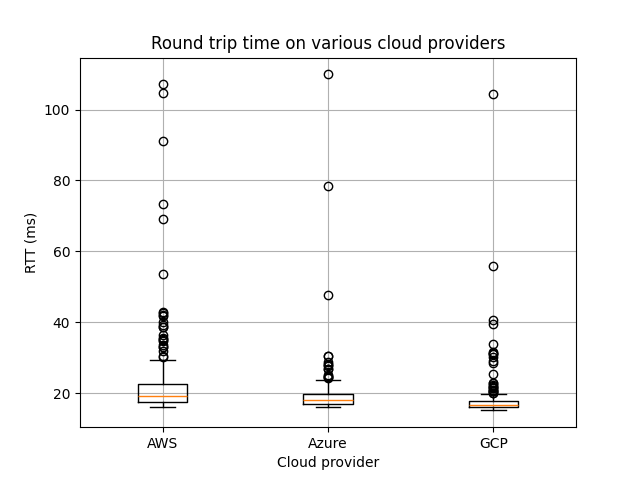
\includegraphics[width=\textwidth]{boxplot.png}
\caption{Box and whisker plot showing the round trip times for each VM}
\label{boxplot}
\end{figure}

\begin{figure}
\label{latency}
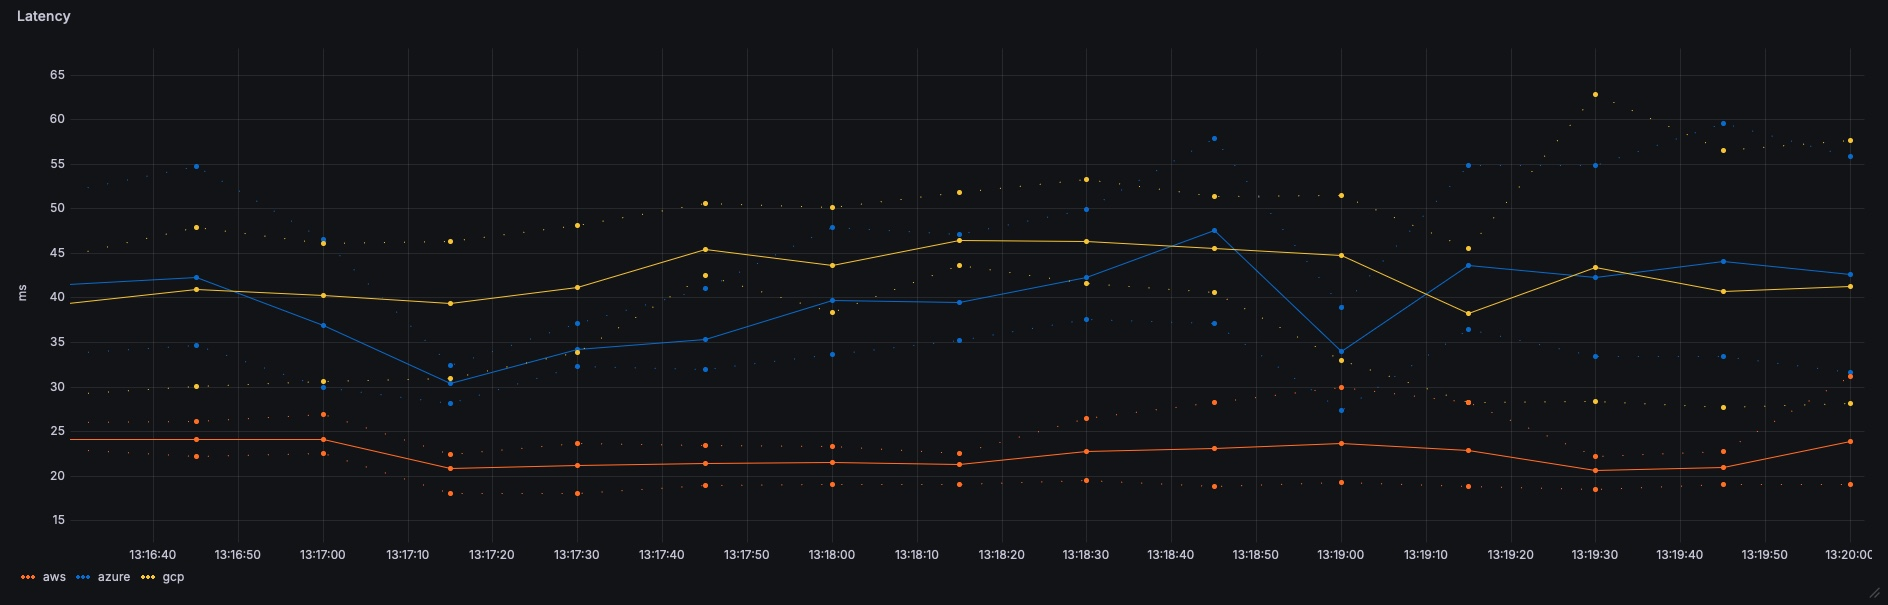
\includegraphics[width=\textwidth]{Latency.jpeg}
\caption{Grafana plot of network latency for each VM}
\end{figure}

\begin{figure}
\label{latency-var}
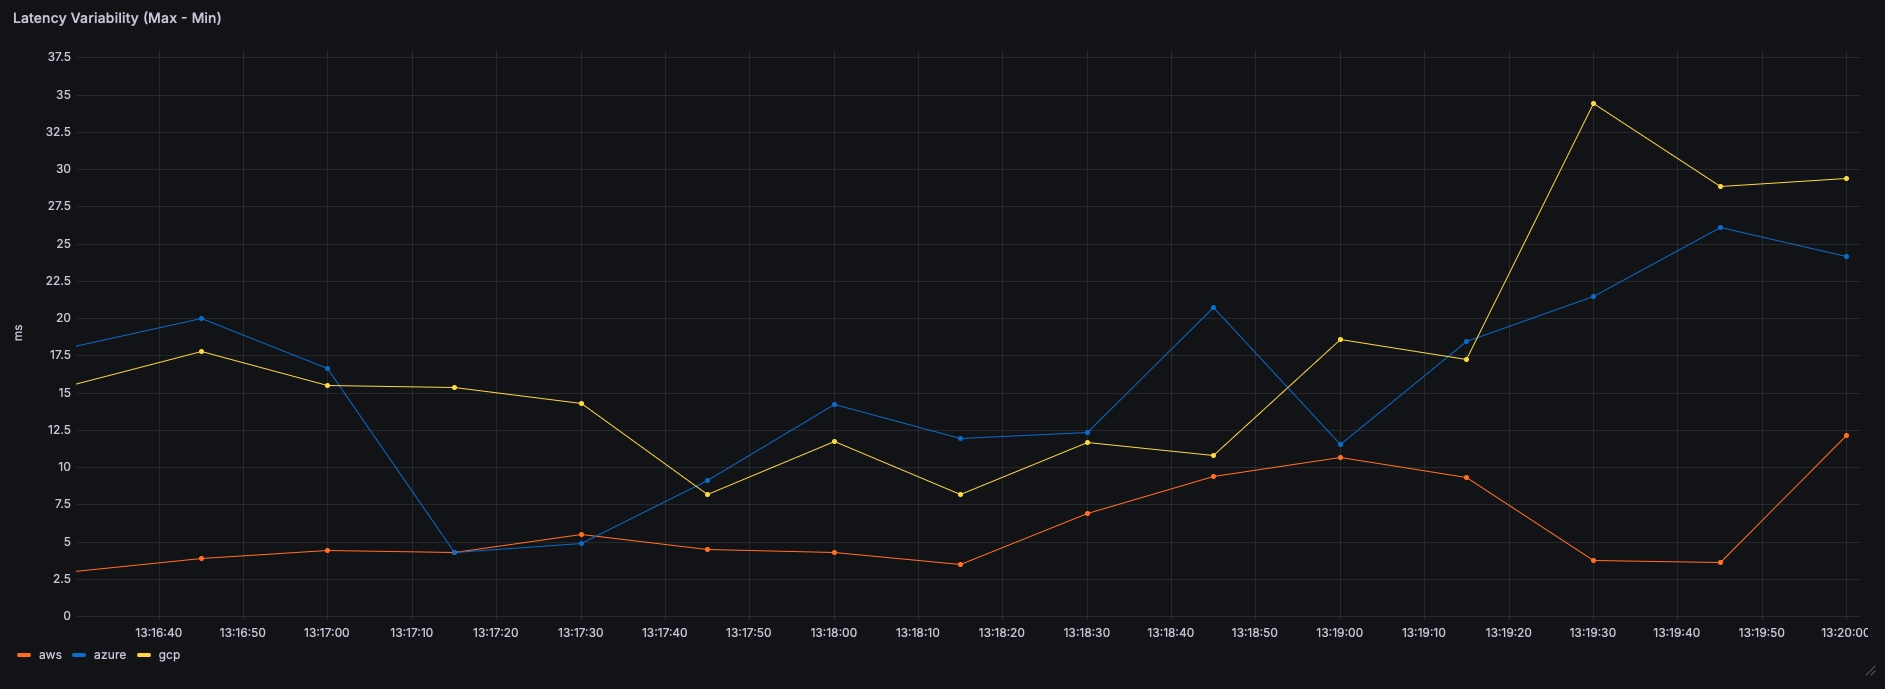
\includegraphics[width=\textwidth]{LatencyVar.jpeg}
\caption{Grafana plot of the variability of the network latency for each VM}
\end{figure}

\Cref{boxplot} shows the RTTs from each cloud provider, here we see that GCP outperforms both AWS and Azure. GCP has lower means, less variance and fewer outliers above 40ms. While GCP has lower RTT than the other providers, \Cref{latency} shows that AWS has consistently lower network latency than both Azure and GCP. As the RTT for GCP was lower than AWS this must mean that the traffic returning from AWS is much slower than traffic returning from GCP. This would be bad for the considered application as players rely on feedback from the server for the game to feel responsive and to inform future decisions. Unfortunately the variability for the latency on GCP is far more inconsistent than the variability experienced with the alternate VMs, spiking near the end of the test to over 3 times its lowest variability (shown in \Cref{latency-var}). Inconsistent latency would cause jitters in gameplay which could ruin the experience for players. This would likely mean that, despite the slower RTT AWS would be the best option purely from a network latency standpoint as its RTTs are mostly comparable to GCP's but AWS has consistently lower variance. Azure is stuck in the middle of GCP and AWS with higher RTT than GCP but higher latency and variance than AWS, this means that, only taking latency/RTT into account, AWS would be the best option for deploying a game.

\begin{figure}
\label{download}
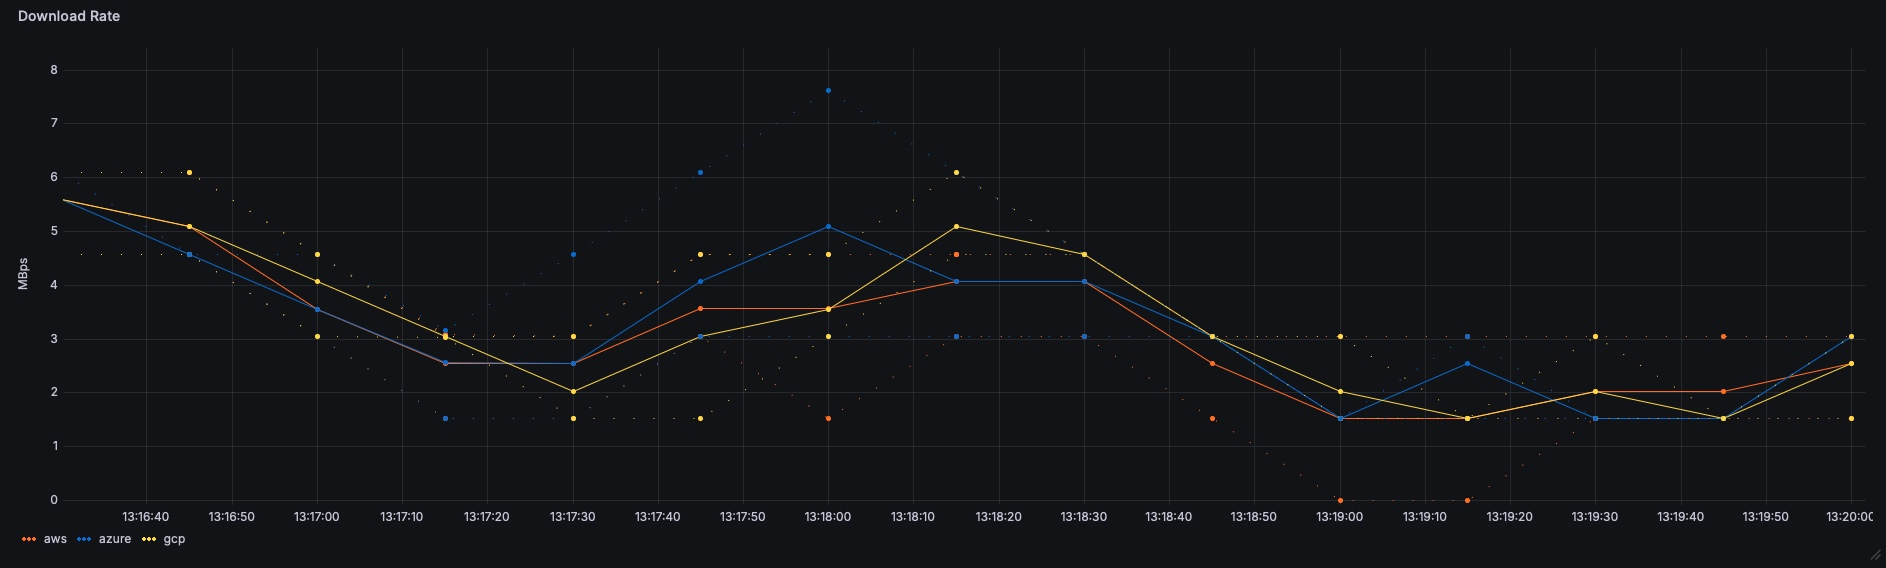
\includegraphics[width=\textwidth]{DownloadRate.jpeg}
\caption{Grafana plot of download rate for each VM}
\end{figure}

\begin{figure}
\label{download-var}
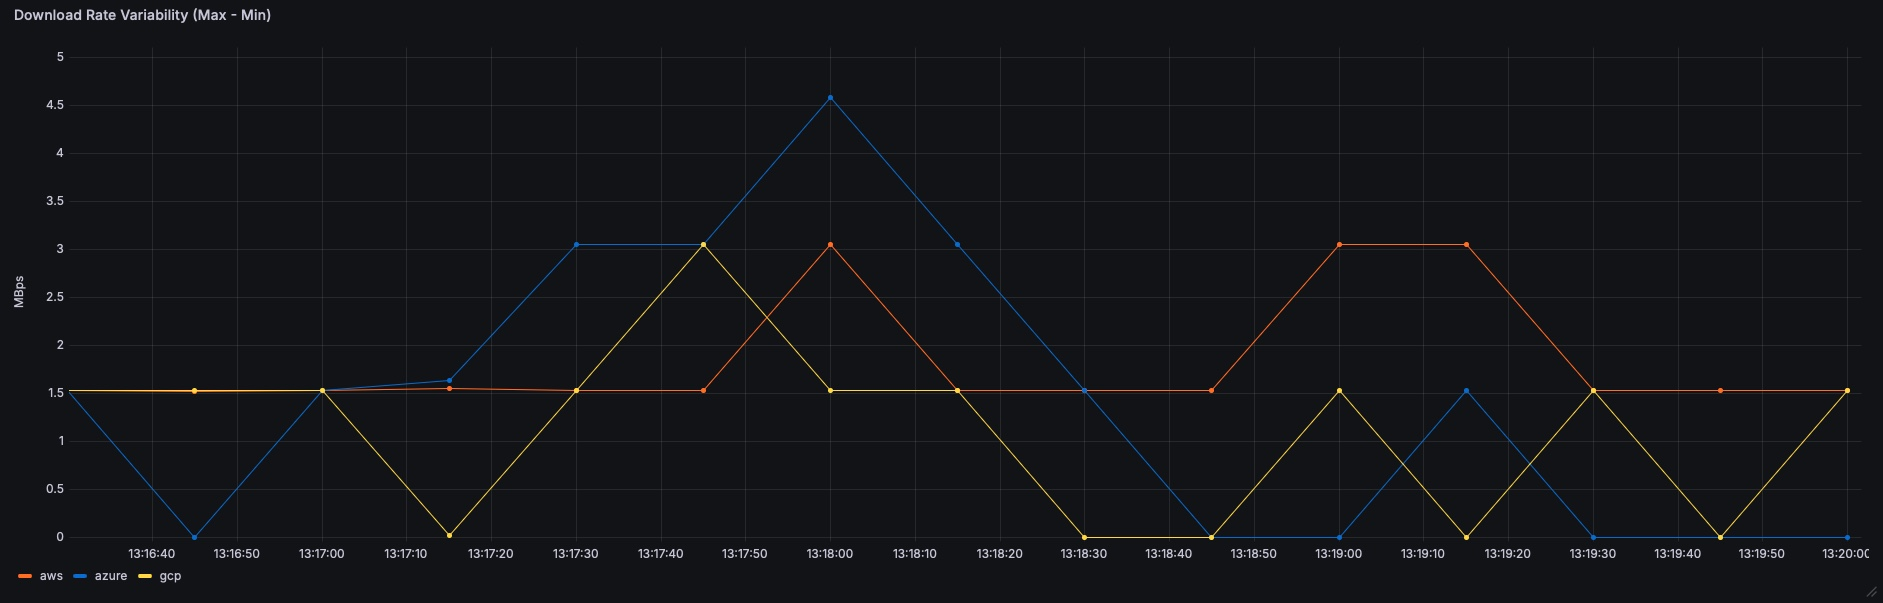
\includegraphics[width=\textwidth]{DownloadRateVar.jpeg}
\caption{Grafana plot of variability of download rate for each VM}
\end{figure}

\begin{figure}
\label{upload}
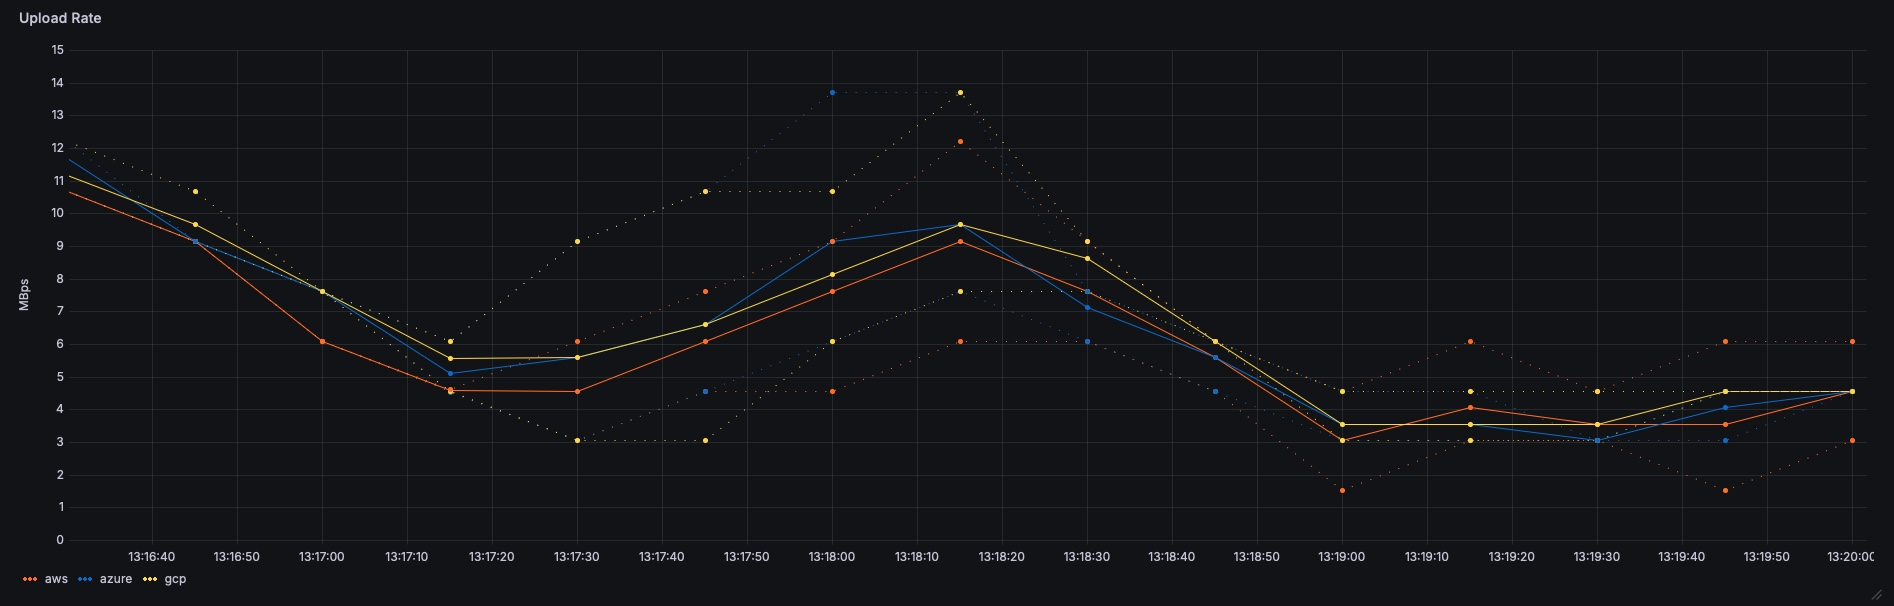
\includegraphics[width=\textwidth]{UploadRate.jpeg}
\caption{Grafana plot of upload rate for each VM}
\end{figure}

\begin{figure}
\label{upload-var}
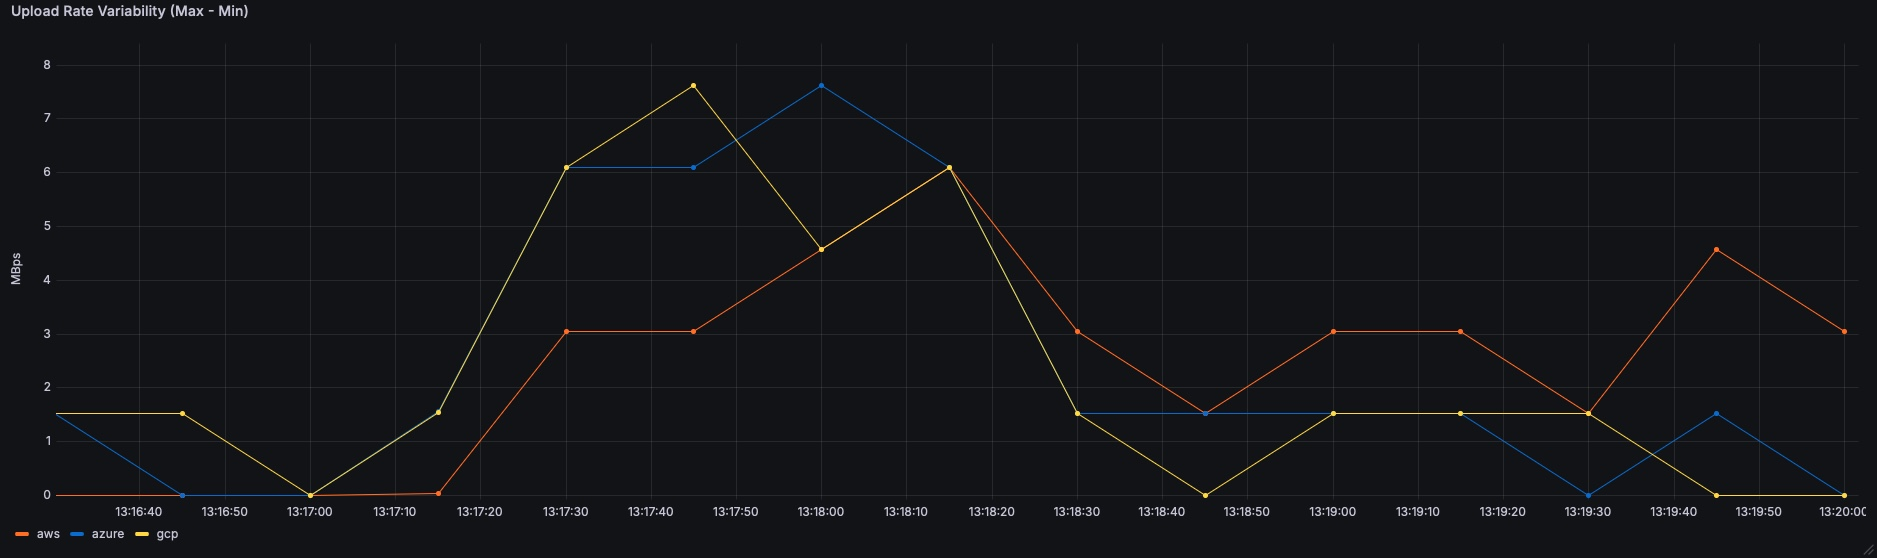
\includegraphics[width=\textwidth]{UploadRateVar.jpeg}
\caption{Grafana plot of variability of upload rate for each VM}
\end{figure}

\section*{Conclusions}

\section*{Appendices}

\subsection*{Code Listings}
\lstinputlisting[caption=Test script, language=bash, label=test-script]{scripts/test.sh}

\lstinputlisting[caption=Benchmarking server, language=Go, label=benchmarking-server]{scripts/main.go}

\lstinputlisting[caption=Box plot for RTT, language=Python, label=boxplot-script]{scripts/ping_boxplot.py}

\end{document}
